\documentclass[../main/main.tex]{subfiles}

\newdate{date}{22}{04}{2020}

\begin{document}

\section{Lecture 13}
 \displaydate{date}. Compiled:  \today. Rachele+Alice.

\subsubsection{Slide 207}

\begin{figure}[h!]
\centering
\includegraphics[page=11,width=0.9\textwidth]{../lessons/pdf_file/12_lesson.pdf}
\end{figure}

In this lesson I'll recap the results we have seen so far regarding the interactions of the quasi-static field which impinges on a set of spherical nanoparticles, which can be considered independent, in the sense that the relative distances between the nanoparticles is so large that single scattering events can be considered, that is the light impinging on each nanoparticle is the same and is the external field and we neglect the additional contribution coming from the scattering field from all the other nanoparticles in the ensemble.

So basically we are describing Lambert-Beer kind of experiment that is we are shining light with a given intensity $I_0$ on a ensemble of nanoparticles embedded in a matrix or in vacuum or any medium provided it is transparent and non absorbing and we are measuring the light coming in the very same direction of propagation of the incoming beam after passing through the thickness of $z$ of our sample.

We have seen that in the single scattering approximation, which holds for reasonable concentration of nanoparticles, we can write the intensity for any given wavelenght of frequency as an exponential decay function, which is:
$$
I(z) = I_0 e^{-\gamma z}
$$
where $\gamma$ is the extinction coeffincient wich is related to the numerical density of the nanoparticle $\rho$ times the cross section of extinction (we remember that the extinction is the sum of two processes: the scattering and absorbtion event which occurs at NP level), which measure the probability of this event to occur.
$k$ is the wavevector of light (of course when we enter a medium of refractive index $n$, we have that $k$ is $k_0 n$ which is nothing else than the wavevector of vacuum times the refractive index of that medium).

As we will see in a moment when we will address the full Mie theory, which handles not only the dipolar approximation but also the fully multipolar approximation, we will see that we are able to re-write the scattering cross-section as this expression  (1) which involves the square modulus of the polarizability $\alpha$ and we will see that in the dipolar approximation this will be proportional to the square of the volume of the nanoparticle. The absorption cross-section (2) is proportional to the imaginary part of the polarizability $\alpha$ which is proportional to the volume.
The extinction cross-section (3) is the sum of the two, so when R $\rightarrow$ 0 the dominant part will be the absorprion cross-section.
With these simple expressions we will see that we can obtain the celebrated form of the scattering absorbition which sum up to the extinction cross section, which reads like that (4)
So in the extinction cross-section we have a term proportional to the volume of the NP (in our case is a spherical NP) times the constant $\epsilon_m^{3/2}$ which is related to the dieletric function of the medium. The term $\omega/c$ tells you about the wavelength in which you are (this is not the $k_0$ value in our system). The most important part is related to the fraction with $\epsilon_2$, which involves the imaginary part at the numerator of the NP dieletric function, and most important at the denominator we just used ?regionalazed? formal complex number since the cross section must be real numbers.
We have  $(\epsilon_1 + 2 \epsilon_m)^2 + (\epsilon_2)^2$ and you can immediatly realized that when the denominator tends to zero because \(  (\epsilon_1 + 2 \epsilon_m)^2 = 0 \), we have a resonance in the cross section \( \sigma _{ext} \) as we have seen for the local field enanchment. Because the last \(  (\epsilon_1 + 2 \epsilon_m)^2 = 0 \) is the Frohlich condition for the resonance in the dipolar regime.

Hence, at the Frohlich condition we have resonance and of course smaller is the imaginary part \( \varepsilon _2 \) the sharper is the resonance of our system.  So \( \varepsilon _2 \) is responsible of the width of the resonance, whereas \( \varepsilon _1 \) is responsible for the spectral position of the resonance in our system.
I would like to stress the fact that the position of the resonance is not a property of the NP itself, but of the combination of the NP plus the medium in which is embedded: it's a metamaterial property, in the sense that is a property that is controlled as the combination of the two materials as we will describe in more details in the following.

\newpage

\subsubsection{Slide 208}

\begin{figure}[h!]
\centering
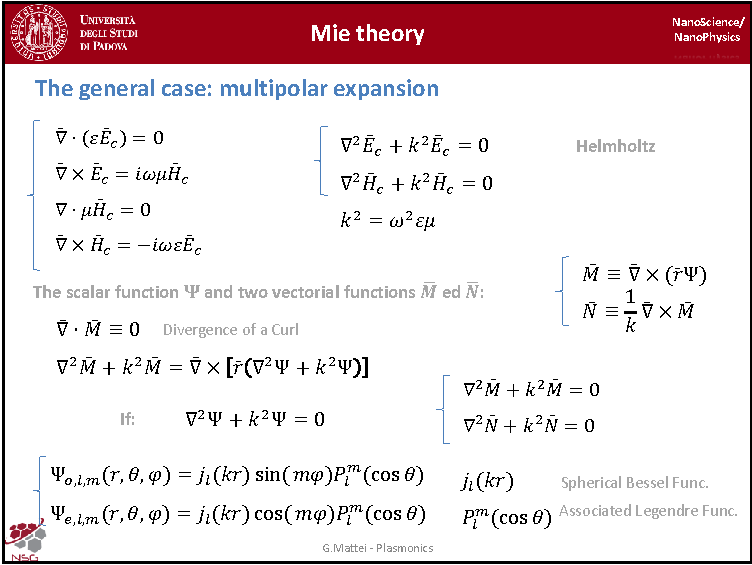
\includegraphics[page=1,width=0.9\textwidth]{../lessons/pdf_file/13_lesson.pdf}
\end{figure}

To address the fully solution which goes beyond the quasi-static or dipolar cases, we need to follow the full Mie theory.
We will just look at the basic concept and we will not enter in details. I would like just to discuss the basic idea of the full Mie theory: we have to solve the fundamental problem for a plane wave impinging on an isolated spherical particle embedded in a non-absorbing medium.

So the major problem is the difference in symmetry between the incoming plane wave and the symmetry of the sphere (NP) which have a spherical geometry.
So we have these two different gemetries which implies a quite complicated changing the symmetry and use of not cartesian description of the wave equation but instead a polar description of them (which complicates a little bit, but you have seen the same tecnique when you have solved hydrogen atoms in quantum mechanics or rigid rotor problem in classical mechanics).

Let us see how Mie attached the problem.
We can start writing the Maxwell equations and you may remember that if we are dealing with complex electric and magnetic field the temporal derivative of any function (which is an harmonic evolving function, a function which evolve with a phase \( i \omega  \)) the derivative is an operator which is multiplied by \( - i \omega  \). If we use this trick we can simplify the notation and se we can rewrite in the harmonic approximation the Maxwell equations for the electric and magnetic fields (the two quantities different from zero). We do not have any free charges or free currents so these two quantities can be setted to zero.
So using equation (2) and (4) we can write the Helmholtz equation for boht the electric and magnetic field. The \( k^2 \) parameter is nothing else \( \omega ^2 \varepsilon  \mu  \) where the quantities \( \varepsilon  \mu  \) can be written:
\begin{itemize}
\item If we are in vacuum: \( \varepsilon _0 \mu _0 \).
\item If we are in a materual: \( \varepsilon_r \varepsilon _0   \) and \( \mu _r \mu _0 \), where \( \varepsilon _r \) and \( \mu _r \) are the relative quantities.
\end{itemize}

So how do we solve the Helmholtz equation? Of course those equation are similar to the wave equations, apart the fact that we have a vector function here, not a scalar function.
So the idea of Mie is to try to recast those equations, moving the solution to an additional function which is a scalar function, a sort of generating function, which is able to generate a basis function for the vectors.
So that in this way we can obtain a vectorial equation of the full basis for the scalar functions when we are solving the classical problem in spherical wave equation in spherical coordinates.

Basically, we want to have the solution in terms of separation of variables, $R$ the radial coordinate, $\theta$  the polar angle and $\phi$ the azimuthal angle, so we separate of the variables so that we can obtain basis for expressing that most general solution in terms of those basis.
Mie is trying to find a scalar function $\Psi$ and two vectorial function $M$ and $N$, which are generated by \( \Psi  \) and which are orthogonal like electric and magnetic field, so we will use this trick to use $M$ and $N$ as a basis with suitable symmetries for the most general form of the electric and magnetic field in complex form.
Of course if we look at the property of these two functions \( M \) and \( N \) we immediatly realize that the divergence of \( M \) is identically 0 because \( M \) is a curl of function, and by definition the divergence of a curl is zero.
This is exactly what we want because in both cases we have the divergence of our fields (magnetic and electric) are both 0.

We will see that \( M \) and \( N \) will obey the very same Helmholtz equation and if you for instance take the curl of the equation (1) you end up in an equation for \( N \) (2), or if you take the curl of equation (2) you end up in the equation (3) which is nothing but the equivalent of the Helmholtz equation for the \( M \) fields, which can be rewritten with algebric manipulation as the curl of these function here and of course, provived that this expression is identically zero, that is if the \( \Psi  \) function satisfy the scalar Helmholtz equation (4) we can obtain that both \( M \) and \( N \) will fullfill the vectorial Helmholtz equation.
So provided that (4) is true, the equations in (5) are also true.

So we have a very simple basis for expanding the most general forms of the electric and magnetic field.
Of course we did this by translating the vectorial equation into a scalar equation. So we need to solve the much more simpler scalar wave equation (we now how to solve that from quantum mechanics).
Using the variable separation, the solution has a radial part, that is the spherical Bessel function, and an angular part which is a function of  $\theta$, $\Phi$ and ${P^m}_l$ (associated Legendre functions).


If we want to solve the scalar equation the scalar equation for \( \Psi  \) (which is the generating scalar function), we can use as a very general representation of the \( \Psi  \) function the basis which are \( \Psi _{o,l,m} \) (odd) or \( \Psi _{e,l,m} \) (even) and which are function of the polar coordinates.


\newpage

\subsubsection{Slide 209}

\begin{figure}[h!]
\centering
\includegraphics[page=2,width=0.9\textwidth]{../lessons/pdf_file/13_lesson.pdf}
\end{figure}

Before proceeding, we can just recall the definition of Spherical harmonics to remind the nature of those functions.
In classical mechanics the factor \( (-1)^m \) is usually absent.
Those functions can be used as a basis for the angular description when you need to solve the wave equations in polar coordinates.
Those functions full-fill the orthonomality condition when are integrated over the solid angle.

Of course, instead of using the complex form, we can use the equivalent real form which is a combination of the two functions with odd and even component of the spherical harmonics.
This is the one showed in the previous slide.

\newpage

\subsubsection{Slide 210}

\begin{figure}[h!]
\centering
\includegraphics[page=3,width=0.9\textwidth]{../lessons/pdf_file/13_lesson.pdf}
\end{figure}

The real part (which will be radial coordinate in our system) is controlled by the spherical Bessel functions. The first three are reported here.
They are oscillating function which fades going toward larger value of the argument.
The spherical Bessel function can be considered as the real part of a more general class of functions: the spherical Hankel functions.


\newpage

\subsubsection{Slide 211}

\begin{figure}[h!]
\centering
\includegraphics[page=4,width=0.9\textwidth]{../lessons/pdf_file/13_lesson.pdf}
\end{figure}

Those functions can be described here. We have the real part and the imaginary part in the two plots. In any case the amplitude of oscillation, with respect to the \( x \) axis, tends to zero when the argument is getting larger.

\newpage

\subsubsection{Slide 212}

\begin{figure}[h!]
\centering
\includegraphics[page=5,width=0.9\textwidth]{../lessons/pdf_file/13_lesson.pdf}
\end{figure}

This is the physical problem that we switch back to: we have a plain wave incoming which is impinging on a spherical particle and we want to obtain information on the scattered and transmitted fields (as we have seen both electrical and magnetic part of the two fields). The easiest part is to use the expansion in vectorial spherical harmonics \( l,M,N \) (which are the vectorial version of the spherical harmonics).
We remember that those (M and N) are generated by the scalar generating function \( \Psi  \) and they have a peculiar symmetry that is the odd and even subscript which remind us that you are taking the \( \sin(\Psi )  \) or the \( \cos(\Psi )  \).  The other numbers \( M_{ol1} \) and \( N_{el1} \) are labels of the basis in terms of the angular function.

Of course, since we are dealing with a plane wave, the temporal evolution in (1) is \( e^{-i \omega t}  \) (and of course it will be unaffected) and since we are assuming for instance that is the plane wave travelling in the \( z \) direction and it is polarized over the \( x \) direction (\( \hat{u}_x  \) is the unity vector in the x direction), the amplitude is \( E_0 \) and \( k  \) is the wave vector in the direction of propagation.
So we have this basic description of the wave nature of the incoming light.
Of course, we need to expand this plane wave in terms of the component with $l$ which can run from 1 to \( \infty  \) and taking $m$ just equal to 1 (so that we can simplify the number of basis that we use in our problem). The fraction is just a normalizing constan. LEt us remind that we are dealing with not imaginary complex version of the fields, when we are dealing with real word or measured quantities we have to take the real part.

The most difficult part is to find similar expression for the scattering and transmitted field.
In this case the simplest consideration that we can do for building the shape of these two fields is that they are in phase (there is no variation in term of the temporal part) and regarding thew spatial part we need to find the scattered and trasmitted field with the very same generating function as the incoming beam (that will set the rules for the symmetry of the fields as we have seen in much more simple quasistatic descrpition of the problem).

So we use expression similar to the previous one but in this case we need to introduce unknown coefficients which are complex number in general.
As soon as we know those coefficient, we can explicitly write the form of the scattered and transmitted fields, as we did for the much simpler case of the dipolar approximation.

Of course, to find them we need to apply the continuity (as we did for the quasi-static approximation) at the surface of the particles of the tangential component of the electric field and continuity of the normal component of the displacement field which is related to the electric field by multiplication by the dielectric function (so when you cross perpendicularly the interface you have a discontinuity in the electric field because you have a continuity of the displacement vectors).

\newpage

\subsubsection{Slide 213}

\begin{figure}[h!]
\centering
\includegraphics[page=6,width=0.9\textwidth]{../lessons/pdf_file/13_lesson.pdf}
\end{figure}

Of course if you apply all this machinary to the problem in a very similar way we have already did in the quasi-static approximation, we end up in a closed form for the coefficient (here instead of $l$ we used $n$, because is more common in recent books), express it in terms of $\mu$ (magnetic permeability of the NP), $m$ (which is the relative refractive index of the nano particles divided by the refractive index of the medium).
The prime sign here indicates derivation with respect to the argument of the functions. \( \mu _1 \) is the magnetic permeability of the medium.

So we can have a closed solution for those coefficients.

\newpage

\subsubsection{Slide 214}

\begin{figure}[h!]
\centering
\includegraphics[page=7,width=0.9\textwidth]{../lessons/pdf_file/13_lesson.pdf}
\end{figure}

We can further simplify this expressions by introducing a new set of functions which are the Riccati-Bessel functions \( \psi _n \) and \( \xi _n \) (1).

In the case in which the two magnetic permeabilities are equal (\( \mu _1 = \mu  \)), so we do not need to consider the magnetic contribution of our nanoparticle (so there is no difference in the magnetic property between the medium and the NP, which is normally the case at optical frequencies so this is very reasonable assumption), we ends up in this form for $a_n$ and $b_n$ coefficients, which control the scattered field in the Mie solution, as a function of the Riccati-Bessel function.
I would like just to show the shape of the first coefficient of this expansion.
For example $a_1$ and $b_1$  involve the dielectric properties of the of the material.  $a_1$  is proportional to the third power of this adimensional number $k$ times R (the size parameter), and so it’s proportional to the volume of the nanoparticle, while $b_1$ is proportional to the fifth power .
$a_1$  is expected to have a resonant behaviour when the Frohlich condition is fulfilled.
More interesting, is the presence of the fraction with the coefficient \( (\varepsilon - \varepsilon _m) \), and you may recognize that is very similar to the coefficient that we used for the solution in the quasi-static regime. So \( a_1 \) is expected to have a resonant behavior provided that the Frohlich condition is fullfilled for our system.
I would like to underline here that the Mie solution is not restricted to metallic nanoparticles but the metallic case is a peculiar, because metals can fulfill the Frohlich condition  in the visible range.

So you realize that the Mie theory is really a giagantic construction, in which mathematical skills are the best and he was able to find these solutions in closed forms.

So when we want to implement those solutions in a computer code, the solution is straight forward: we need just to implement the analytic shape of the coefficient. So we can build the electric and magnetic fields scattered or trasmitted in the NP straightforwardly, so we can immeaditly have access to the near field properties (as we have seen) and also to the far field properties (because from \( E \) and \( H \) field we can build the pointing vector, and if we calculate the flux of the pointing vector we can obtain information on the power distribution in the space and so we can compute the extinction cross section building it as the sum of absorbition and scattering cross section).

\newpage

\subsubsection{Slide 215}

\begin{figure}[h!]
\centering
\includegraphics[page=8,width=0.9\textwidth]{../lessons/pdf_file/13_lesson.pdf}
\end{figure}

Indeed, Mie solved this complex problem and he was able to show that the scattering cross section can be written as the expression (1), which involves the square modulus of the \( a_l \) and \( b_l \) coefficients, whereas the extinction cross section can be written as in (2) (the infinite sum over all multipolarities of the real part of \( a_l  \) and \( b_l \)). Of course the absorbition cross section can be calculated as the difference between the two.
The coefficient in fron of all the cross sections involves \( k^2 \), which is as the usual expression is the wave vector in the medium and can be written in terms of the \( k_0 \) (that is the wave vector in vacuum) times the refractive index of the medium (which is a non-dispersive medium, otherwise we cannot compute the cross section in the way that we have introduced in the previous lesson).

Using this result we can see that the $a_l$  and $b_l$ component are proportional to the size coefficient \( k R \) parameter elevated to a suitable power of \( l \). So when the size parameter is going to 0 (basically when the radius is much smaller than the wavelength),  $a_l$  dominates over $b_l$ of course, because it involves a lower power of the coefficient.
For that reason, the component of the extinction cross-section when the size parameter tends to zero,
is dominated by the lower power of the size parameter, that is the absorption cross-section dominates over the scattering cross-section (which on the contrary involves the square modulus of the coefficients).
On the contrary, when the size parameter will be larger, we see that scattering is dominating over absorption, according with the multipolarity in our system.

\newpage

\subsubsection{Slide 216}

\begin{figure}[h!]
\centering
\includegraphics[page=9,width=0.9\textwidth]{../lessons/pdf_file/13_lesson.pdf}
\end{figure}

To see this, we can compute (or simulate) the scattering extinction and absorbition cross-section with the full Mie theory. We can immediately see that the blue cuve is the shape of the extinction cross-section for gold nanoparticles in silica. We see that four radius of \( 5nm \) of gold into silica (with refractive index of \( n=1.46 \), so it is not absorbing so perfectly fullfill the requirement of the Mie theory). There is a black curve, which is the absorbition cross-section, which is exactly superimposed to the one of the extinction cross section (blue one), because the scattering contribution to be seen (red curve) needs to be amplified by two orders of magnitude. The red curve is the amplified scattering cross-section, so we can see that is perfectly negligible.

So, when the size  of the nanoparticle is small, the extinction is dominated by absorption and not by the scattering.


In this plot I used the  cross-section normalized by the volume, which is another way to represent the ccross-section in order to reduce the difference when you compare cross-sections for nanoparticles with different size. We could have used also the efficiency
by normalize the cross-section not by the volume but by the geometric shadow of the nanoparticles (which is the area projected perpendicularly to the direction of motion of the plale wave).

\newpage

\subsubsection{Slide 217}

\begin{figure}[h!]
\centering
\includegraphics[page=10,width=0.9\textwidth]{../lessons/pdf_file/13_lesson.pdf}
\end{figure}

If we look at the shape of the resonances when the size is larger (so when the radius is \( R=5nm \)), also in this case we have gold nanoparticles in silica, and we see much better that there is a resonant behavior and that scattering and absorbition are more balanced with respect to the previous case. You can immediately see  that, for such kind of particles, scattering and absorption are both relevat to obtain the global properties of our nanosystem.

By the way, with this result, we can have a clear understanding the problem from which we start this discussion, that is the colour of the Lycurgus cup. Yoy may remembert that the colour of the Lycurgus cup was  green when looking at ambient light but red when illuminated by light coming from the internal of the cup (different reflecting and transmittance proprierties). That is when we look at the transmittance properties of the Lycurgus cup, we see the cup red, on the contrary, when we look at the scattered light we see the green color emerging.

The Mie theory is able to give a simple expanation of this phenomenon that was not understood befor its theory.

Let us see how we can explain the color of the Lycurgus cup with the simple graph here.
\begin{itemize}
\item Indeed, if we have for instance light which is given by ambient light illuminating the Lycurgus cup, we need to simply look at the light which is scattered in the environment from the nanoparticles. Of course, the most important cross section for this process is the scattering cross-section plotted in red.
Remember that in the Lycurgus gas you have an alloy of nanoparticles of gold and silver, but you have seen that the scattering property is similar, indeed when you have a composition of the two you have a cross-section which is more or less in between those of two separated system. So the explanation that we can give for the Lycurgus cup is qualitatively similar to the one that we can give with purely gold nanoparticles. Of  course, you see that in this case the scattering cross-section has a peak in the green portion of our spectrum (I reported here the colour spectrum in the visible range). You see that in this case the peak of the scattering cross-section is around the green (of course in the case of the alloy, we will be slightly blue-shift, but of course still in the green range of the colours). If we have metallic nanoparticles in the Lycurgus cup, we need to expect a colour which is dominated by the green. If you decompose the entire spectrum in RGB, the red, green, blue  contribution to the colour emergin from nanoparticles is dominated by the green. Of course both red and blue are of the same level, and they will give a much smaller contribution to the whole colour which is dominated by the green.

\item Of course when we are looking at the light trasmitted through the Lycurgus cup, the most important process that we are looking is the extinction cross-section, because we are looking at both absorbtion of light and scattering of light with respect to the direction of motion (of arrival of the incoming beam). So if we look at the extinction cross-section of course we see that the largest part of the light which does not reach our eyes is the green component, and the second component which is scattered out of our system (because of the absorbtion) is the blue component, whereas the red component is unaffected by our system.

So it is clear that the color will be dominated by the spectral component which is less affected by the interaction with the nanoparticles, which is the red. So four that reason we will see the red colour of the Lycurgus cup in trasmittance.

\end{itemize}
So we have obtained a very simple explanation by this very complex theory of Mie in our case. In the following we will look at the other properties that can be obtained by the Mie theory in much more details.


\clearpage


\end{document}
